% Slide 1 — TurtleBot Mecanum holonome
\subsubsection{Turtlebots}

\begin{frame}{Le robot TurtleBot Mecanum}
\begin{columns}[T]
  \begin{column}{0.6\textwidth}
    \begin{itemize}
      \item Plateforme mobile holonome grâce aux roues Mecanum:
        \begin{itemize}
          \item Roues à galets inclinés permettant translations dans toutes les directions et rotation sur place.
          \item Combinaison des vitesses des 4 roues pour générer $v_x$, $v_y$ et $\omega$.
        \end{itemize}
      \item Composition matérielle: Raspberry Pi 4, carte OpenCR, moteurs Dynamixel, batterie LiPo 3S.
      \item Communication et contrôle: micro-ROS (USB/série) et Wi-Fi
    \end{itemize}
  \end{column}
  \begin{column}{0.4\textwidth}
    \begin{figure}
      \centering
      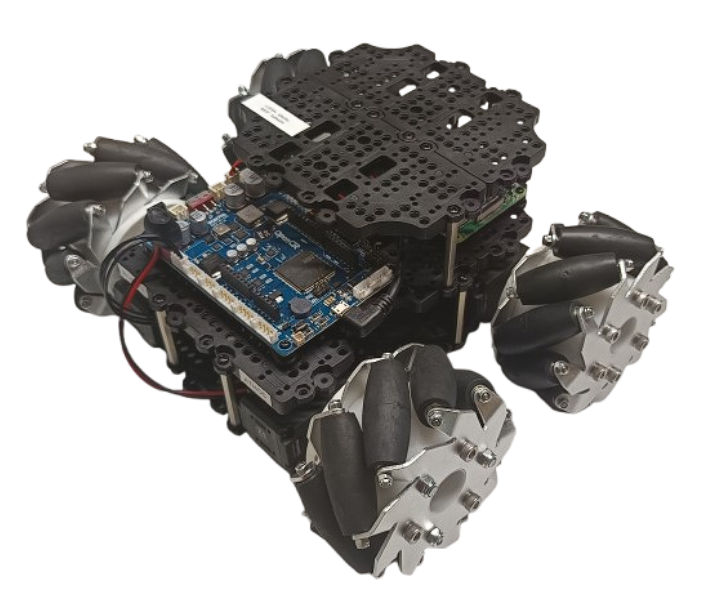
\includegraphics[width=\textwidth]{5-Descriptions-realisations/outils/pic/Mecanum.png} % Mettez le bon chemin vers votre image
      \caption{Robot TurtleBot Mecanum.}
    \end{figure}
  \end{column}
\end{columns}
\end{frame}

% Slide 2 — Configurations des robots
\begin{frame}{Configurations des robots TurtleBot Mecanum}
  \small
  \begin{table}
  \centering
  \caption{Configurations matérielles et logicielles des robots}
  \begin{tabular}{|l|l|l|l|l|}
    \hline
    Robot & Ubuntu & RAM (Go) & CPU & Stockage (Go) \\
    \hline
    Aramis & 22.04 Desktop & 4 & 64-bit quad-core & 32 \\
    Athos & 22.04 Desktop & 4 & 64-bit quad-core & 32 \\
    Porthos & 22.04 Desktop & 4 & 64-bit quad-core & 32 \\
    d'Artagnan & 22.04 Server & 2 & 64-bit quad-core & 16 \\
    Edmon & 22.04 Server & 2 & 64-bit quad-core & 16 \\
    Mercedes & 22.04 Server & 2 & 64-bit quad-core & 16 \\
    \hline
  \end{tabular}
  \end{table}
\end{frame}
